\documentclass[conference]{IEEEtran}
\IEEEoverridecommandlockouts
\usepackage{listings}
\usepackage{xcolor}
\usepackage{hyperref}
\usepackage{amsthm}
\usepackage{pgfplots}
\usepackage{graphicx}
\graphicspath{ {./time_comp/} }
\lstset { %
    language=C++,
    backgroundcolor=\color{black!5}, % set backgroundcolor
    basicstyle=\footnotesize,% basic font setting
}
%New colors defined below
\definecolor{codegreen}{rgb}{0,0.6,0}
\definecolor{codegray}{rgb}{0.5,0.5,0.5}
\definecolor{codepurple}{rgb}{0.58,0,0.82}
\definecolor{backcolour}{rgb}{0.95,0.95,0.92}

%Code listing style named "mystyle"
\lstdefinestyle{mystyle}{
  backgroundcolor=\color{backcolour},   commentstyle=\color{codegreen},
  keywordstyle=\color{magenta},
  numberstyle=\tiny\color{codegray},
  stringstyle=\color{codepurple},
  basicstyle=\ttfamily\footnotesize,
  breakatwhitespace=false,         
  breaklines=true,                 
  captionpos=b,                    
  keepspaces=true,                 
  numbers=left,                    
  numbersep=5pt,                  
  showspaces=false,                
  showstringspaces=false,
  showtabs=false,                  
  tabsize=2
}

%"mystyle" code listing set
\lstset{style=mystyle}
% The preceding line is only needed to identify funding in the first footnote. If that is unneeded, please comment it out.
\usepackage{cite}
\usepackage{amsmath,amssymb,amsfonts}
\usepackage{algorithmic}
\usepackage{graphicx}
\usepackage{textcomp}
\usepackage{xcolor}
\def\BibTeX{{\rm B\kern-.05em{\sc i\kern-.025em b}\kern-.08em
    T\kern-.1667em\lower.7ex\hbox{E}\kern-.125emX}}
\begin{document}

\title{IIIT Allahabad\\DAA Assignment-05\\
}

\author{\IEEEauthorblockN{Sanket Kokude}
\IEEEauthorblockA{\textit{IIB2019034} \\
}
\and
\IEEEauthorblockN{Harshit Kumar}
\IEEEauthorblockA{\textit{IIB2019035} \\
}
\and
\IEEEauthorblockN{Viful Nirala}
\IEEEauthorblockA{\textit{IIB2019036} \\
}
}

\maketitle

\begin{abstract}
In this report we designed a Dynamic Programming algorithm to find the number of subsets of given array having a particular XOR value.

\end{abstract}

\section{Introduction}
Given an array arr[] of size n ,we used dynamic programming approach to find the number of subsets having XOR value as K.\\
%%Here in dp[i][j] we keep a count of number of sets from 0 to i-1 having XOR value as j.At the end the program we will give dp[n][k] as output.\\
Dynamic Programming (DP) is an algorithmic technique for solving an optimization problem by breaking it down into simpler subproblems and utilizing the fact that the optimal solution to the overall problem depends upon the optimal solution to its subproblems.


\section{Algorithm Design}
Following is Dynamic Programming algorithm :

\begin{itemize}
\item  First we find a number m, which is actually the maximum value any XOR subset can acquire. We define a number m such that $m = pow(2,(log2(max(arr))+1)) – 1$. 
\item After that check whether the given k is greater or not if it is then return 0. 
\item After that create a 2D array $dp[n+1][m+1]$, such that $dp[i][j]$ equals to the number of subsets having XOR value j from subsets of $arr[0…i-1].$
\item We initialize all values of dp[i][j] as 0.
\item Set value of dp[0][0] = 1 since XOR of an empty set is 0.
\item Iterate over all the values of $arr[i]$ from left to right and for each $arr[i]$, iterate over all the possible values of XOR i.e from 0 to m (both inclusive) and fill the $dp$ array as following:\\
      for i = 1 to n:
       
           \quad for j = 0 to m:
          
             \quad \quad \quad \quad $dp[i][j] = dp[i-1][j] + dp[i-1][j {\oplus} arr[i-1]]$\\
             
                   
\item This can be explained as, if there is a subset arr[0…i-2] with XOR value j, then there also exists a subset arr[0…i-1] with XOR value j also if there exists a subset arr[0….i-2] with XOR value $j \oplus arr[i]$ then clearly there exist a subset arr[0…i-1] with XOR value j, as:\\
$j \oplus arr[i-1] \oplus arr[i-1] = j$.\\

\item Counting the number of subsets with XOR value k: Since dp[i][j] is the number of subsets having j as XOR value from the subsets of arr[0..i-1], then the number of subsets from set arr[0..n] having XOR value as K will be dp[n][K].
\end{itemize}

\section{Algorithm and illustration}
Suppose a given array is $arr=[6,2,4,3,5]$ and $K=4$.\\
Then find a number m which is the maximum value any XOR subset can have by \\
$m = 2^{log_2(max(arr))+1)}$ – $1$\\
as $max(arr)=6$\\
$m = 2^{log_26+1}$ – $1$\\
$m=7$\\
%Let's take a array $arr=[1,2,3,4]$ and K=6\\
Then initialise $dp$ (2D array  $dp[n+1][m+1]$) with all values as 0 where $n= sizeof(arr)$ i.e $n=5$.\\
$dp[0][0]=1 $(Empty set)\\\\
So $dp$ matrix will be
$$
\begin{bmatrix}
1 & 0 & 0 & 0 & 0 & 0 & 0 & 0\\
0 & 0 & 0 & 0 & 0 & 0 & 0 & 0\\
0 & 0 & 0 & 0 & 0 & 0 & 0 & 0\\
0 & 0 & 0 & 0 & 0 & 0 & 0 & 0\\
0 & 0 & 0 & 0 & 0 & 0 & 0 & 0\\
0 & 0 & 0 & 0 & 0 & 0 & 0 & 0\\
\quad 
\end{bmatrix}
$$
\\
Now we Iterate over all values of arr[i] from i=1 to i=n.Then for each iteration ,we also iterate over all values of XOR.\\\\
dp(After 1st Iteration):\\
$$
\begin{bmatrix}
1 & 0 & 0 & 0 & 0 & 0 & 0 & 0\\
1 & 0 & 0 & 0 & 0 & 0 & 1 & 0\\
0 & 0 & 0 & 0 & 0 & 0 & 0 & 0\\
0 & 0 & 0 & 0 & 0 & 0 & 0 & 0\\
0 & 0 & 0 & 0 & 0 & 0 & 0 & 0\\
0 & 0 & 0 & 0 & 0 & 0 & 0 & 0\\
\quad
\end{bmatrix}
$$
\\
dp(After 2nd Iteration):\\
$$
\begin{bmatrix}
1 & 0 & 0 & 0 & 0 & 0 & 0 & 0\\
1 & 0 & 0 & 0 & 0 & 0 & 1 & 0\\
1 & 0 & 1 & 0 & 1 & 0 & 1 & 0\\
0 & 0 & 0 & 0 & 0 & 0 & 0 & 0\\
0 & 0 & 0 & 0 & 0 & 0 & 0 & 0\\
0 & 0 & 0 & 0 & 0 & 0 & 0 & 0\\
\quad
\end{bmatrix}
$$
\\
dp(After 3rd Iteration):\\
$$
\begin{bmatrix}
1 & 0 & 0 & 0 & 0 & 0 & 0 & 0\\
1 & 0 & 0 & 0 & 0 & 0 & 1 & 0\\
1 & 0 & 1 & 0 & 1 & 0 & 1 & 0\\
2 & 0 & 2 & 0 & 2 & 0 & 2 & 0\\
0 & 0 & 0 & 0 & 0 & 0 & 0 & 0\\
0 & 0 & 0 & 0 & 0 & 0 & 0 & 0\\
\quad
\end{bmatrix}
$$
\\
dp(After 4th Iteration):\\
$$
\begin{bmatrix}
1 & 0 & 0 & 0 & 0 & 0 & 0 & 0\\
1 & 0 & 0 & 0 & 0 & 0 & 1 & 0\\
1 & 0 & 1 & 0 & 1 & 0 & 1 & 0\\
2 & 0 & 2 & 0 & 2 & 0 & 2 & 0\\
2 & 2 & 2 & 2 & 2 & 2 & 2 & 2\\
0 & 0 & 0 & 0 & 0 & 0 & 0 & 0\\
\quad
\end{bmatrix}
$$
dp(After 5th Iteration):\\
$$
\begin{bmatrix}
1 & 0 & 0 & 0 & 0 & 0 & 0 & 0\\
1 & 0 & 0 & 0 & 0 & 0 & 1 & 0\\
1 & 0 & 1 & 0 & 1 & 0 & 1 & 0\\
2 & 0 & 2 & 0 & 2 & 0 & 2 & 0\\
2 & 2 & 2 & 2 & 2 & 2 & 2 & 2\\
4 & 4 & 4 & 4 & 4 & 4 & 4 & 4\\
\quad
\end{bmatrix}
$$
Hence, number of subsets having XOR value k is   $dp[n][k]=dp[5][4]=4$.

\section{Algorithm Analysis}
\textbf{Time complexity:}
We are iterating over whole array one by one finding and storing the count of possible subsets that generate a XOR value $j$ (we say) and store it in the $dp[i][j]$ which will need time to iterate over the array of size $n$ and for each element a loop of time complexity $m$ will be iterated.\\

\quad $m=2^{[log_2(max-element)] + 1}-1$\\\\
This will result in the time complexity of \textbf{$O(n*m)$}. 
\\\\
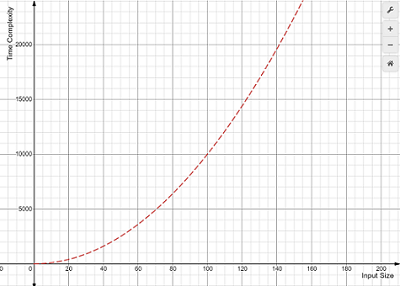
\includegraphics{time_comp}
\textbf{Space complexity:}
In this  approach we will have to store the values for all possible cases that are generated, as the $dp[i][j]$ requires $dp[i-1][j]$ and hence a 2D array of size $n*m$ is required.\\\\
This will result in the space complexity of $O(n*m)$. \\\\


\section{Conclusion}
We can observe that in Dynamic Programming Approach it may consume more space (i.e.$O(1)$ in case of brute force) but will have better time-complexity than Brute force approach(i.e.$O(2^n)$ in case of brute force).
%%Brute Force approach O(2n): One naive approach is to generate all the 2n subsets and count all the subsets having XOR value K, but this approach will not be efficient for large values of n.

 \section{References}
\color{blue}1.{\url{https://www.geeksforgeeks.org/calculate-xor-1-n/} }\\
2. {\url{https://www.geeksforgeeks.org/dynamic-programming/}}\\
3. Cormen, Leiserson, Rivest, and Stein (2009). Introduction to Algorithms, 3rd edition.

\color{black}
\
\begin{titlepage}
    \begin{center}
        \Huge
        \section*{Appendix}
        \end{center}
         \textbf{Code for implementation of this paper is given below:}
\begin{lstlisting}[language=C++,caption=Code for this paper]
#include<bits/stdc++.h>
using namespace std;

int n,k,max_ele=0;

int subsetXOR(int arr[])
{
	// Maximum possible XOR value
	int m = (1 << (int)(log2(max_ele) + 1)) - 1;

	if( k > m )
	    return 0;

	int dp[n+1][m+1];
	// Initializing all the values of dp[i][j] as 0
	for (int i=0; i<=n; i++)
		for (int j=0; j<=m; j++)
			dp[i][j] = 0;

	// The xor of empty subset is 0
	dp[0][0] = 1;

	for (int i=1; i<=n; i++){
		for (int j=0; j<=m; j++){
            dp[i][j] = dp[i-1][j] + dp[i-1][j^arr[i-1]];
            // cout<<dp[i][j]<<" ";
        }
        // cout<<"\n";
    }
	return dp[n][k];
}

int main()
{
    cout<<"Enter the size of array : ";
    cin>>n;
    int arr[n];
    cout<<"Enter the array : ";
    for(int i=0;i<n;i++){
        cin>>arr[i];
        if (arr[i] > max_ele)
		    max_ele = arr[i];
    }
    cout<<"Enter the XOR value :";
    cin>>k;
	cout << "Count of subsets is " << subsetXOR(arr);
	return 0;
}
   
\end{lstlisting}
\end{titlepage}
\end{document}
